\chapter{Fejlesztői dokumentáció}
\label{ch:dev}

\section{Bevezetés}

Az alkalmazáshoz való technológiák kiválasztásakor fontos mind a felhasználó, mind a fejlesztő igényeit figyelembe venni. Szerencsére, jelen esetben van megoldás, amely minden oldal számára a legtöbb kényelmet nyújtja, mégpedig a webalkalmazás. A felhasználó számára könnyű elérést, platformfüggetlenséget, és egy megszokott felületet hordoz magával, ami különösen fontos egy oktatási céllal rendelkező alkalmazásnál, hiszen még kevesebb akadályt helyez a felhasználó és a "tananyag" közé. Fejlesztői szempontból is kényelmes egy ilyen alkalmazást a böngészőre írni, hiszen a JavaScript ökoszisztémában könyvtárak és keretrendszerek tömkelege áll rendelkezésre, melyek segítségével gyorsan és hatékonyan lehet egy webalkalmazást fejleszteni.

\section{Adatforrás}

Az adatok a BKK\nomenclature{BKK}{Budapesti Közlekedési Központ} által szolgáltatott OpenData Portálon\cite{bkkopendata} nyilvánosan elérhető adatbázisból származnak. Az adatokat a BKK a GTFS\index{GTFS -- General Transit Feed Specification} (General Transit Feed Specification) formátumban teszik elérhetővé, ami egy Google-nél kifejlesztett\cite{gtfsabout} nyilvánosan elérhető specifikáció, mely egy szabványos formátumot definiál a tömegközlekedési adatok szolgáltatására.

\section{Tervezés és követelmények}

\subsection{Nem funkcionális követelmények}

\subsubsection{Termék követelmények}

\begin{enumerate}
    \item Hatékonyság
    \begin{compactitem}     
        \item A szoftver kezdeti megnyitásakor legkésőbb 5 másodperc alatt teljesen betöltődik és használhatóvá válik
        \item A szoftver általános használat közben folyamatosan, megakadás nélkül fut egy középkategóriás számítógépen, egy modern böngészőben
        \begin{compactitem}     
            \item Kivétel ez alól az animált útvonaltervezés, amelynek a futása közben a szoftver akadozhat, de nem annyira, hogy használhatatlanná váljon, vagy megakadályozza az animáció leállítását
        \end{compactitem}
        \item A backend válaszideje API hívásokra nem több, mint 5 másodperc (bármilyen lehetséges, érvényes API hívásra)
        \item A szoftver felhasználói bevitelre adott válasz ideje nem több, mint 100 ezredmásodperc
        \begin{compactitem}     
            \item Ebbe beleértendő a betöltést jelző válasz, amíg az alkalmazás API hívásokra várakozik
        \end{compactitem}
        \item A szoftver nem használ a szükségesnél több processzorkapacitást (pl. nem használja processzortól függetlenül az összes elérhető teljesítményt)
    \end{compactitem}
    \item Megbízhatóság
    \begin{compactitem}
        \item A szoftverben ne legyen olyan egyszerűen előidézhető vagy gyakran bekövetkező hibajelenség, ami előfordulása esetén ellehetetleníti vagy jelentősen megnehezíti a szoftver használatát
    \end{compactitem}
    \item Biztonság
    \begin{compactitem}
        \item A szoftver ne tároljon felhasználói adatokat
        \item A szoftver ne tároljon érzékeny adatokat
        \item A szoftver ne tároljon jelszavakat
    \end{compactitem}
    \item Hordozhatóság
    \begin{compactitem}
        \item A szoftver kliens oldala bármilyen WebGL-t támogató modern böngészőben fut, különös tekintettel a Chromium alapú böngészőkre
        \item A szoftver a kliens oldalon állandó, stabil internetkapcsolatot és a szerverrel való kapcsolatot igényel
        \item A szoftver szerver oldala az adatok letöltéséhez stabil internetkapcsolatot igényel, ezt követően csak a klienssel szükséges kommunikálnia
    \end{compactitem}
    \item Felhasználhatóság
    \begin{compactitem}
        \item A szoftver intuitív és könnyen használható
        \item A szoftver kliens oldalának a használatához nem szükséges külön telepítés, komoly számítógépes tapasztalattal nem rendelkező felhasználók számára is egyértelmű
        \item A weboldal felülete egy átlagos számítógéphasználó számára külső segítség nélkül elsajátítható, amennyiben ismerik a szoftver által bemutatott útkereső algoritmusokat
        \item A szoftver szerver oldalának az üzemeltetése hálózati és Docker-compose ismereteket igényel
    \end{compactitem}
\end{enumerate}

\subsubsection{Menedzselési követelmények}

\begin{enumerate}
    \item Környezeti
    \begin{compactitem}
        \item A szoftver kliens oldalon egy egeret és egy billentyűzetet igényel
        \item A szoftver szerver oldalának a futtatásához legalább egy középkategóriás számítógépnek megfelelő hardver szükséges, eltekintve a perifériáktól
    \end{compactitem}
    \item Működési
    \begin{compactitem}
        \item A szoftver legfeljebb egy órás összefüggő időtartamokban lesz használva a kliens oldalon
        \item A szerver oldalon a szoftver folyamatosan fut, legfeljebb 4-5 naponta lehet szükséges karbantartási műveleteket végezni rajta, pl. a szoftver újraindítása (eltekintve az adatforrások frissítésétől)
    \end{compactitem}
    \item Fejlesztési
    \begin{compactitem}
        \item  Frontenden Node.js, React, TypeScript
        \begin{compactitem}
            \item  Térkép és adatok megjelenítéséhez deck.gl, react-map-gl
        \end{compactitem}
        \item  Backenden Node.js, Express, TypeScript
        \begin{compactitem}
            \item  REST API szerver
            \item  SQLite adatbázis
            \item  Adatok importálásához node-gtfs
        \end{compactitem}
        \item  Visual Studio Code fejlesztői környezet
        \item  Docker
        \item  64-bit architektúra
        \item  Verziókezeléshez Git kliens
    \end{compactitem}
    \item Fenntartási
    \begin{compactitem}
        \item Minden API végpont tesztelve és OpenAPI 3 formátumban dokumentálva van
    \end{compactitem}
\end{enumerate}

\subsubsection{Külső követelmények}

\begin{compactitem}
    \item A szoftverhez felhasznált külső forrásból származó médiafájlok jogtiszták
    \item A szoftver nem tartalmaz erkölcsileg megkérdőjelezhető, sértő tartalmat
\end{compactitem}

\subsection{Funkcionális követelmények}

\subsubsection{Funkciók}

\begin{enumerate}
    \item Útkeresés két megálló között budapesti tömegközlekedési járatokon
    \begin{itemize}
        \item Beállítások megadása
        \begin{itemize}
            \item Indulási és érkezési megálló kiválasztása
            \item Indulási idő megadása
            \item Útvonaltervezési algoritmus kiválasztása
            \begin{compactenum}
                \item BFS keresés
                \item Dijkstra algoritmus
                \item Mohó algoritmus
                \item A* algoritmus
            \end{compactenum}
            \item Útvonaltervezési algoritmus paramétereinek megadása
            \begin{compactitem}
                \item Maximális sétatávolság átszállások között
                \item A* algoritmus esetén: heurisztika súlyozása
            \end{compactitem}
        \end{itemize}
        \item Útvonaltervezés
        \begin{itemize}
            \item Algoritmus léptetése
            \item Algoritmus futtatásának indítása
            \item Algoritmus futtatásának szüneteltetése
            \item Algoritmus futtatásának folytatása
            \item Algoritmus visszaállítása alapállapotba
            \item Algoritmus eredményének megjelenítése
            \begin{compactitem}
                \item Potenciális útvonalak megjelenítése a térképen
                \item Soron következő megállók megjelenítése
            \end{compactitem}
        \end{itemize}
    \end{itemize}
\end{enumerate}

\subsection{Felhasználási eset diagram}

A program felhasználói eseteit a \ref{fig:use-case} ábra mutatja be.

\begin{figure}[H]
    \centering
    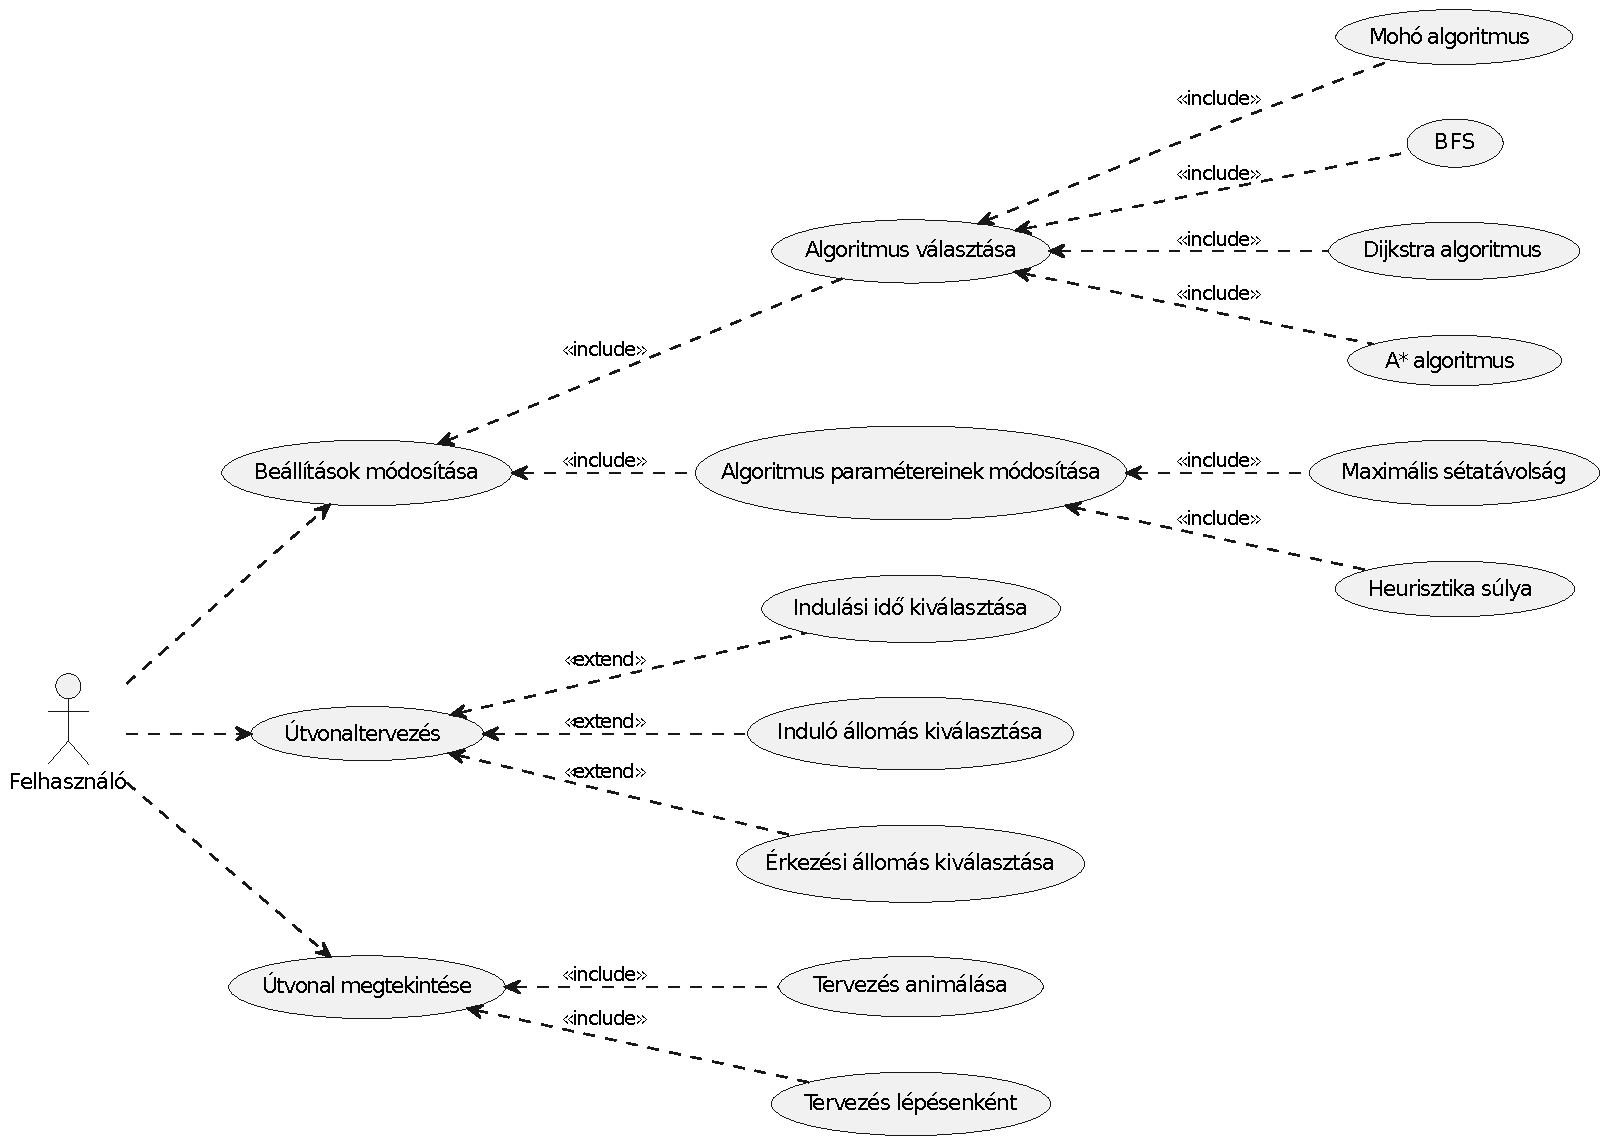
\includegraphics[width=1\textwidth]{use_case}
    \caption{Felhasználási eset diagram}
    \label{fig:use-case}
\end{figure}

\subsection{Felhasználói történet}

A felhasználói történetek a \ref{tab:user-stories-algorithm}., \ref{tab:user-stories-route}., \ref{tab:user-stories-parameters}., és a \ref{tab:user-stories-control}. táblákban olvashatóak.

\begin{table}[H]
    \centering
    \begin{tabular}{|c|c|p{10cm}|}
        \hline
        \textbf{1}  
        & AS A          & Felhasználó \\ \hline
        & I WANT TO     & Megváltoztatni a használt algoritmust \\ \hline
        & SO THAT       & Más algoritmusok vizualizációját tekintsem meg \\ \hline
        \hline
        1 & GIVEN   & A "beállítások" fül van kiválasztva \\ \hline
        & WHEN    & A legördülő menüben a \textbf{BFS algoritmust} választom \\ \hline
        & THEN    & Az útvonaltervezés a \textbf{BFS algoritmussal} fog történni \\ \hline
        \hline
        2 & GIVEN   & A "beállítások" fül van kiválasztva \\ \hline
        & WHEN    & A legördülő menüben a \textbf{Mohó algoritmust} választom \\ \hline
        & THEN    & Az útvonaltervezés a \textbf{Mohó algoritmussal} fog történni \\ \hline
        \hline
        3 & GIVEN   & A "beállítások" fül van kiválasztva \\ \hline
        & WHEN    & A legördülő menüben az \textbf{A* algoritmust} választom \\ \hline
        & THEN    & Az útvonaltervezés \textbf{A* algoritmussal} fog történni \\ \hline
        \hline
        4 & GIVEN   & A "beállítások" fül van kiválasztva \\ \hline
        & WHEN    & A legördülő menüben a \textbf{Dijkstra algoritmust} választom \\ \hline
        & THEN    & Az útvonaltervezés a \textbf{Dijkstra algoritmussal} fog történni \\ \hline
    \end{tabular}
    \caption{Felhasználói történet: algoritmus választása}
    \label{tab:user-stories-algorithm}
\end{table}

\begin{table}[H]
    \centering
    \begin{tabular}{|c|c|p{10cm}|}
    \hline
    \textbf{2}
    & AS A          & Felhasználó \\ \hline
    & I WANT TO     & Kiválasztani az tervezendő útvonalat \\ \hline
    & SO THAT       & Megtekinthetem az útvonaltervezést a választott útvonalon \\ \hline
    \hline
    1 & GIVEN   & A "beállítások" fül van kiválasztva \\ \hline
    & WHEN    & Az "indulási állomás" mezőbe beírom egy állomás nevét \\ \hline
    & THEN    & Az útvonaltervezés a kiválasztott állomástól fog indulni \\ \hline
    \hline
    2 & GIVEN   & A "beállítások" fül van kiválasztva \\ \hline
    & WHEN    & Az "érkezési állomás" mezőbe beírom egy állomás nevét \\ \hline
    & THEN    & Az útvonaltervezés a kiválasztott állomást fogja megkeresni \\ \hline
    \hline
    3 & GIVEN   & A "beállítások" fül van kiválasztva \\ \hline
    & WHEN    & Az "indulási idő" mezőben kiválasztok egy időt \\ \hline
    & THEN    & Az útvonal első járata a kiválasztott idő után fog indulni \\ \hline
    \end{tabular}
    \caption{Felhasználói történet: útvonal kiválasztása}
    \label{tab:user-stories-route}
\end{table}

\begin{table}[H]
    \centering
    \begin{tabular}{|c|c|p{10cm}|}
        \hline
        \textbf{3}
        & AS A          & Felhasználó \\ \hline
        & I WANT TO     & Megváltoztatni a használt algoritmus paramétereit \\ \hline
        & SO THAT       & Más paraméterekkel tekintsem meg az útvonaltervezést \\ \hline
        \hline
        1 & GIVEN & A "beállítások" fül van kiválasztva \\ \hline
        & AND     & Az A* algoritmus van kiválasztva \\ \hline
        & WHEN    & A "heurisztika súlya" mezőben módosítom a súlyt \\ \hline
        & THEN    & Az útvonaltervezés a választott súlyt fogja használni \\ \hline
        \hline
        2 & GIVEN & A "beállítások" fül van kiválasztva \\ \hline
        & WHEN    & A "gyalogos távolság" mezőben módosítom a távolságot \\ \hline
        & THEN    & Az algoritmus által tervezett útvonal részeként nem fog szerepelni
                    két járat között olyan átszállás, ami a megadottnál nagyobb távolságú \\ \hline
    \end{tabular}
    \caption{Felhasználói történet: algoritmus paramétereinek módosítása}
    \label{tab:user-stories-parameters}
\end{table}

\begin{table}[H]
    \centering
    \begin{tabular}{|c|c|p{10cm}|}
        \hline
        \textbf{4}
        & AS A          & Felhasználó \\ \hline
        & I WANT TO     & Interaktívan megtekinteni a tervezett útvonalat \\ \hline
        & SO THAT       & Láthatom az útvonaltervezés lépéseit \\ \hline
        \hline
        1 & GIVEN   & Az "útvonal" fül van kiválasztva \\ \hline
        & AND     & Válaszottam indulási állomást, érkezési állomást és indulási időt \\ \hline
        & AND     & Az algoritmus még nem talált utat a kiválasztott állomások között \\ \hline
        & WHEN    & A "következő lépés" gombra kattintok \\ \hline
        & THEN    & Az algoritmus elvégzi a következő lépését \\ \hline
        \hline
        2 & GIVEN   & Az "útvonal" fül van kiválasztva \\ \hline
        & AND     & Válaszottam indulási állomást, érkezési állomást és indulási időt \\ \hline
        & AND     & Az algoritmus még nem talált utat a kiválasztott állomások között \\ \hline
        & WHEN    & Az "animáció indítása" gombra kattintok \\ \hline
        & THEN    & Az algoritmus addig fut, amíg nem találja meg a cél állomást, vagy nem szüneteltetem \\ \hline
        \hline
        3 & GIVEN   & Az "útvonal" fül van kiválasztva \\ \hline
        & AND     & Az algoritmus az "animáció indítása" gombra való kattintás hatására fut \\ \hline
        & WHEN    & Az "animáció szüneteltetése" gombra kattintok \\ \hline
        & THEN    & A program további interakció nélkül nem végez több lépést \\ \hline
        \hline
        4 & GIVEN   & Az "útvonal" fül van kiválasztva \\ \hline
        & AND     & Az algoritmus talált utat a kiválasztott állomások között \\ \hline
        & WHEN    & A "visszaállítás" gombra kattintok \\ \hline
        & THEN    & Az algoritmus "elfelejti" a talált utat és megállókat, és az alapállapotába áll \\ \hline
    \end{tabular}
    \caption{Felhasználói történet: Algoritmus irányítása}
    \label{tab:user-stories-control}
\end{table}

\subsection{Felhasználói felület tervek}

Az alkalmazás nyitóoldala a \ref{fig:wireframe-settings}. ábrán látható.

\begin{figure}[H]
    \centering
    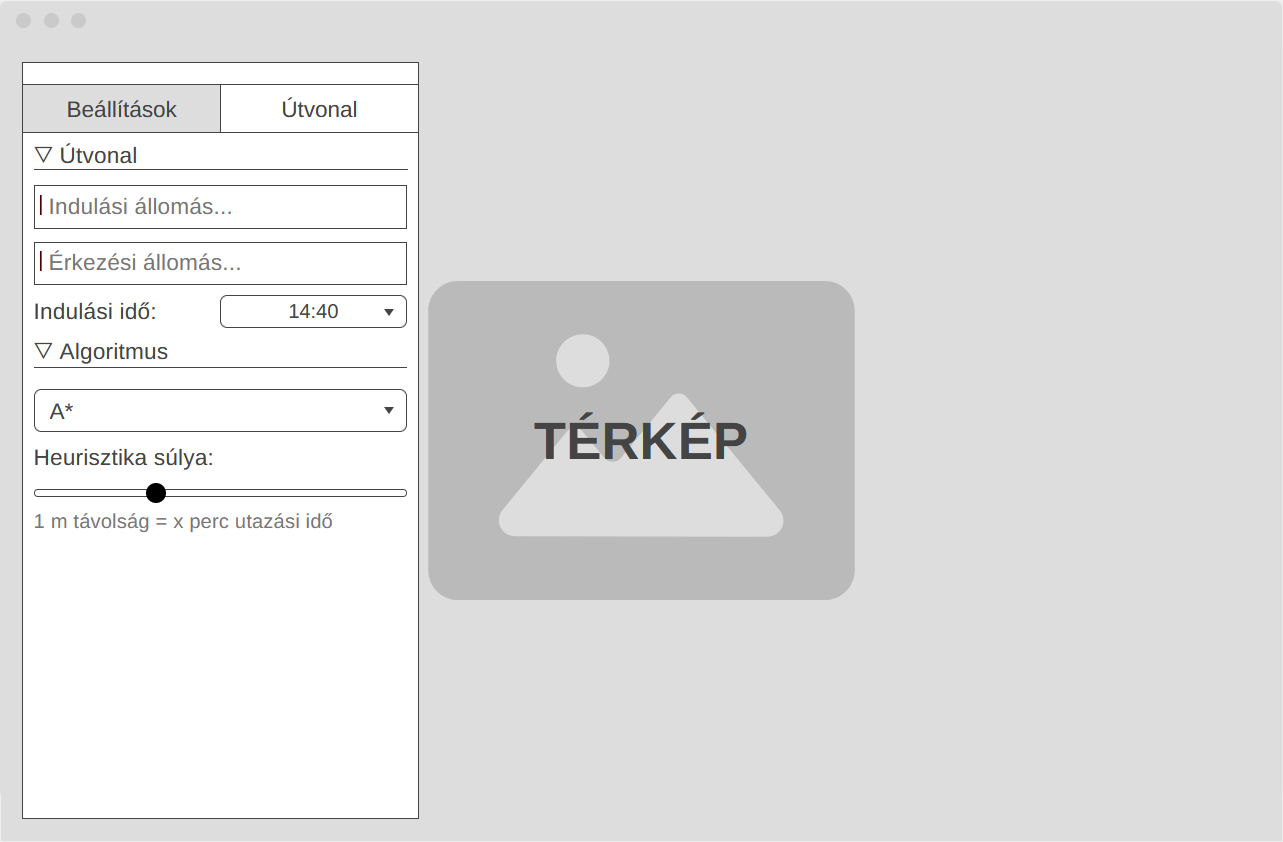
\includegraphics[width=1\textwidth]{wireframe_settings}
    \caption{Beállítások felület terve}
    \label{fig:wireframe-settings}
\end{figure}

Innen az "indulási állomás" és az "érkezési állomás" mezőkbe beírva egy állomás nevének a részletét rákereshetünk arra, és kiválaszthatjuk azt. A keresési találatok megjelenítését a \ref{fig:wireframe-search}. ábra mutatja be.

\begin{figure}[H]
    \centering
    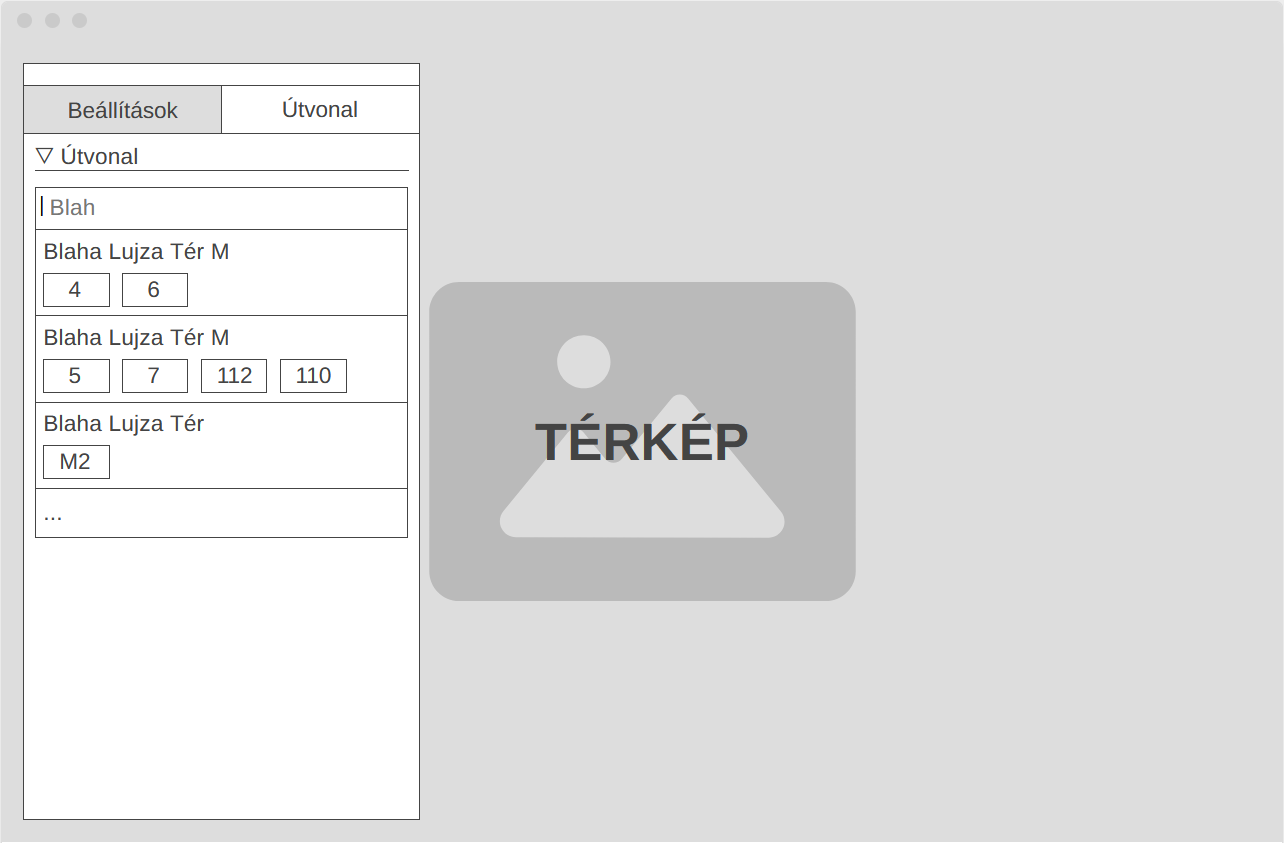
\includegraphics[width=1\textwidth]{wireframe_search}
    \caption{Megálló keresésének felület terve}
    \label{fig:wireframe-search}
\end{figure}

Ezen állomások kiválasztása után az "indulási idő" mezőben kiválaszthatjuk az indulási időt (vagy az alapértelmezettet használhatjuk), majd az "útvonal" gombra kattintva a \ref{fig:wireframe-plan}. ábrán látható felületen irányíthatjuk az algoritmus futását, és tekinthetjük meg annak állapotát és eredményét.

\begin{figure}[H]
    \centering
    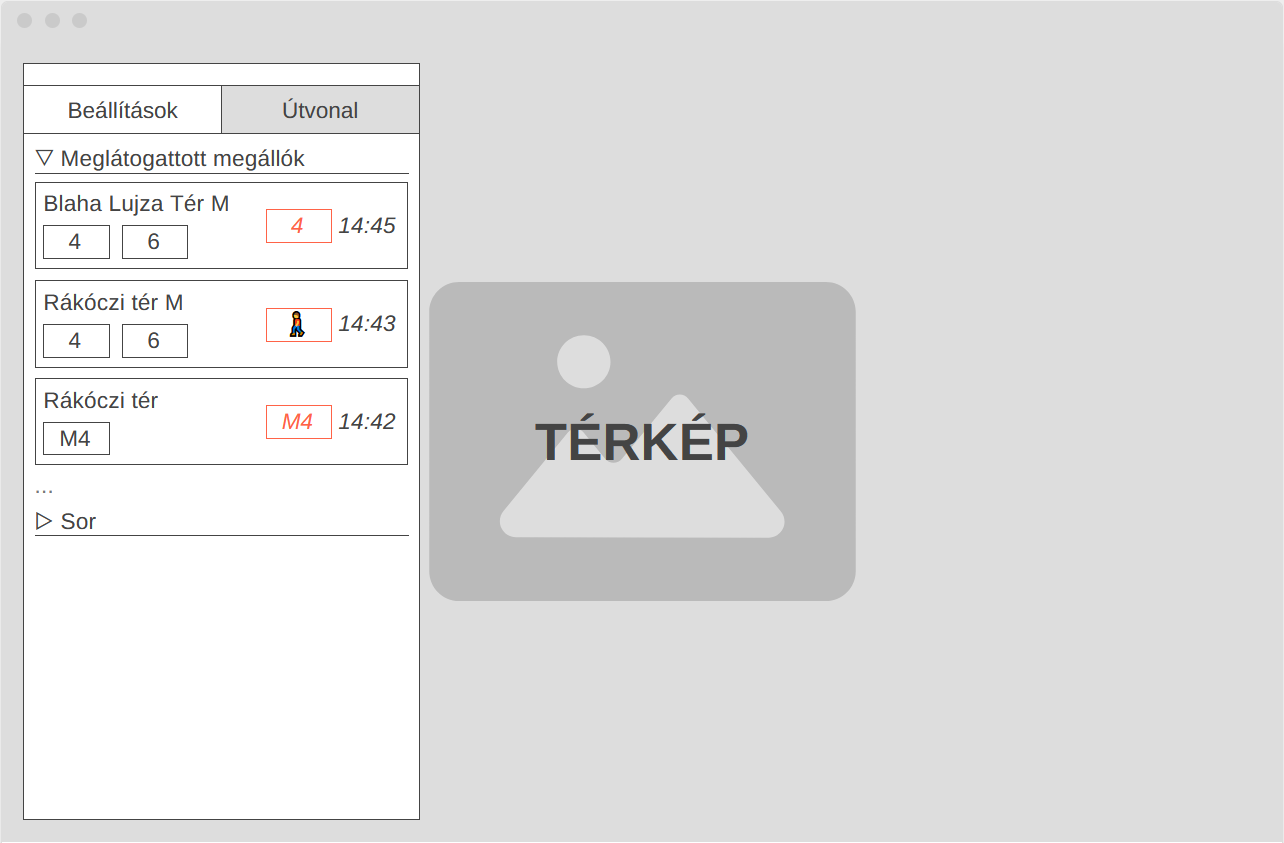
\includegraphics[width=1\textwidth]{wireframe_plan}
    \caption{Algoritmus irányításának felület terve}
    \label{fig:wireframe-plan}
\end{figure}

\section{Magas szintű áttekintés}

\subsection{Alkalmazás felépítése}

Az alkalmazás egy backendből és egy frontendből áll, REST API-n\nomenclature{REST}{REpresentational State Transfer, egy szoftverarchitektúra típus, ami megkötésekkel garantálja többek között az adatok gyorsítótárazhatóságát\cite{rest}} keresztül kommunikálnak egymással. A backend feladata a GTFS formátumban elérhető adatok adatbázisba való betöltése, valamit ezen adatok szolgáltatása a frontend számára. A frontend egy webalkalmazás, mely a felhasználói felületet biztosítja a felhasználók számára.

Fontos megemlíteni, hogy az útvonal tervezése és az algoritmusok futtatása a frontenden történik. Azért választottam ezt a megoldást, hogy az API-n átvitt adatok komplexitását minimalizáljam; mivel a frontendnek egyébként is szüksége van az összes információra az algoritmus belső állapotáról, így a számításokat a frontendre helyezve elég az adatbázis-lekérdezéseket és azok eredményét kommunikálni a kettő között.

\subsection{Verziókövetés}

A változtatásokat \textit{git} használatával tartom számon, így a fejlesztés során bármikor visszaállítható egy korábbi verzió, vagy összehasonlítható két verzió közötti különbség.

\subsection{Backend áttekintés}

% \footnote{A \textit{Node.js} egy platform, ami JavaScript kód szerveroldali futtatását teszi lehetővé}
A backend egy \textit{Node.js} alapú alkalmazás, mely az \textit{Express.js} keretrendszert használja a REST API megvalósítására. Fontos tényező volt a környezet kiválasztásában, hogy az NPM\footnote{Az NPM egy csomagnyilvántartás JavaScript csomagoknak, saját állításuk szerint a világ legnagyobb csomagnyilvántartása\cite{nodeabout}}-en megtalálható \textit{node-gtfs}\cite{nodegtfs} csomag egyike volt a kevés elérhető könyvtáraknak\footnote{A GTFS adatok feldolgozására való könyvtárak listája megtalálható a \url{https://gtfs.org/resources/gtfs/} oldalon \textit(Letöltés dátuma: 2024.11.22.)}, amelyek képesek GTFS adatok adatbázisba való betöltésére és lekérdezésére. További előnye a \textit{Node.js} backend választásának, hogy a frontenddel azonos a fejlesztői környezet, így a fejlesztéshez nem kell új programokat telepíteni, és a frontend és a backend fejlesztése közötti váltást is egyszerűvé teszi.

Hogy a backend akár távoli szerveren is egyszerűen beindítható legyen a teljes tesztkörnyezet reprodukálása nélkül, az alkalmazást Dockerizáljuk\index{Docker -- virtualizációs technológia, mely alkalmazások platformfüggetlen futtatását teszi lehetővé}; így egy \texttt{git clone [repo] \&\& docker compose up -d} paranccsal bárhol egyszerűen futtatható a backend (ahol a Docker és a git telepítve van).

% \footnote{A TypeScript egy nyelv, ami a JavaScriptre épül, de statikus típusokat is támogat\cite{typescript}}
Az olvashatóság és karbantarthatóság érdekében a backend kódja TypeScript nyelven íródik.

\subsection{Frontend áttekintés}

A frontend egy \textit{React} webalkalmazás, mely a backendhez hasonlóan \textit{TypeScript} nyelven van írva. A \textit{React} egy komponens alapú könyvtár, melynek segítségével a felhasználói felületet kisebb, önállóan működő komponensekre bonthatjuk, így a kód olvashatóbb és karbantarthatóbb lesz. Azért erre esett a választásom Angular és Vue helyett, mert a React népszerűsége messze túlszárnyalja ezekét\cite{reactcomparison}, így a fejlesztők számára könnyen elérhetőek a segédanyagok és a közösség támogatása is.

Az utak térképen való megjelenítéséhez a két fő lehetőség a \textit{deck.gl}, és az erre épülő\cite{kepler} \textit{kepler.gl}, amit az Ubernél fejlesztettek nagy volumenű utazási adat megjelenítésére. A döntésem a \textit{deck.gl}-re esett, mert egyszerű utak és megállók megjelenítésére szükségtelen a \textit{kepler.gl} komplexitása, illetve a \textit{deck.gl} dokumentációját is részletesebbnek és könnyebben érthetőnek találtam. A React választása melletti érv volt az is, hogy a \textit{deck.gl} a Reacthoz biztosít előre elkészített komponenseket (más könyvtárakkal ellentétben), így a két technológia jól egymásra épül.

\subsection{Fejlesztői környezet felállítása}

Az alkalmazás fejlesztéséhez a következő programok telepítése szükséges:

\begin{compactitem}
    \item \textit{Node.js (és npm csomagkezelő)}: Bár a backend és a frontend is futtatható Dockerben, az Intellisense számára érdemes a host gépen is telepíteni a használt csomagokat.
    \item \textit{Docker}
    \item \textit{git}
    \item \textit{IDE/szövegszerkesztő}: Én a Visual Studio Code-ot használom és javaslom, de használható más IDE (pl. WebStorm) is.
\end{compactitem}

Függőségek telepítéséhez a backend és a frontend mappákban a \texttt{npm install} parancsot kell futtatni.

\subsection{Alkalmazás futtatása}
\label{sec:run-app}

Az alkalmazást fejlesztéshez is Dockerben futtatjuk, hogy a program írásakor feltételezhessük, hogy mindig ugyanaz a környezet áll rendelkezésre. A Dockerfile a frontend és a backend esetében egyaránt négy stage-et tartalmaz:

\begin{compactenum}
    \item \texttt{base}: Az alap image, amely `node:lts-alpine`-t használ. Erre épül az összes többi stage.
    \item \texttt{development}: Az \texttt{npm run dev} parancsot futtatja. Ennek a futtatásakor az alkalmazás figyeli a fájlrendszert\footnote{A fájlrendszer figyeléséről frontend esetén a \textit{vite}, backend esetén a \textit{tsx} gondoskodik.}, és újraindítja a kódot minden alkalommal, amikor egy fájl frissül (frontenden csak azokat a komponenseket, amiket érinti a frissítés --- ezt HMR-nek, azaz Hot Module Replacement-nek hívják\cite{hmr}).
    \item \texttt{build}: Az \texttt{npm run build} parancsot futtatja, ami JavaScript-re fordítja a TypeScript kódot.
    \item \texttt{production}: A \texttt{build}-ből lemásolja a lefordított kódot és futtatja azt.
\end{compactenum}

A stage-ek külön bontásának köszönhetően a \texttt{production} image a lehető legkisebb lesz, és a Docker építéskor gyorsítótárban tudja tárolni a lépések közös elemeit. A különválasztott fejlesztői és a telepítési környezetnek megfelelően két külön Docker Compose fájl is található a projektben: a \texttt{docker-compose.debug.yml} a fejlesztői környezetet állítja fel, míg a \texttt{docker-compose.yml} a telepítési környezetet. Az indításkor az ennek megfelelő parancs használandó (\ref{src:compose-dev}).

\lstset{caption={Alkalmazás indítása különböző konfigurációkban}, label=src:compose-dev}
\begin{lstlisting}[language={bash}]
    # Fejlesztői környezet indítása
    docker compose -f docker-compose.debug.yml up -d --build

    # Telepítési környezet indítása
    docker compose up -d --build
\end{lstlisting}

Bár telepítési környezethez minden adott, hogy Dockerből futtatható legyen az alkalmazás mindkét része, a frontend statikusan kiszolgálható fájlokra fordul le, így ezt nem érdemes egy Docker konténerben futtatni. Ehelyett javasolt az \texttt{npm run build} által a \textit{dist} könyvtárba lefordított fájlokat egy webszerveren keresztül kiszolgálni, például Nginx vagy Apache HTTP szerver segítségével.

\section{Backend}

\subsection{Könyvtárszerkezet}

A backend könyvtárszerkezete a következő:

\begin{compactitem}
    \item \texttt{src/}: A forráskódokat tartalmazó könyvtár, aminek a tartalma fordításra kerül.
    \item \texttt{src/configs/}: Futásidőben használt konfigurációs fájlok helye.
    \item \texttt{src/models/}: Adatbázis sémák helye.
    \item \texttt{src/routes/}: A REST API végpontokat tartalmazó fájlok.
    \item \texttt{src/utils/}: Segédfüggvények adatok betöltésére és lekérdezésére.
    \item \texttt{src/index.ts}: Az alkalmazás belépési pontja.
    \item \texttt{test/}: Teszteléshez szükséges fájlok.
    \item \texttt{.dockerignore}: \texttt{.gitignore}-hoz hasonlóan a Docker által figyelmen kívül hagyott fájlok listája.
    \item \texttt{Dockerfile}: A Docker image felépítéséhez szükséges fájl.
    \item \texttt{drizzle.config.ts}: A \textit{drizzle-kit} konfigurációs fájlja (részletek: \ref{sec:database}).
    \item \texttt{package.json}: A függőségeket és egyéb metainformációkat tartalmazó fájl.
    \item \texttt{package-lock.json}: Az \texttt{npm} csomagkezelő által generált fájl, mely a telepített függőségek pontos verzióit tartalmazza.
    \item \texttt{generate-types.ts}: Segédscript, mely az adatbázis sémából TypeScript típusokat generál a frontend számára.
    \item \texttt{tsconfig.json}: A TypeScript konfigurációs fájl.
\end{compactitem}

\subsection{Adatbázis}
\label{sec:database}

A program indításakor az első lépés az adatbázis létrehozása és feltöltése a GTFS adatokkal. Az adatok betöltésére és lekérdezésére a korábban említett \textit{node-gtfs} csomagot használom. (NPM-en és kódban egyszerűen \textit{gtfs}-nek hívják, korábban a GitHub-on szereplő nevét használtam a szabványtól való megkülönböztetés végett. A továbbiakban kisbetűvel írva, gtfs-ként fogok hivatkozni rá.)

A gtfs a GTFS adatokat egy SQLite adatbázisba tölti be, melynek sémája a GTFS specifikációban meghatározott táblákat tartalmazza (\ref{fig:gtfs-schema}). 

\pagebreak

\begin{figure}[H]
    \centering
    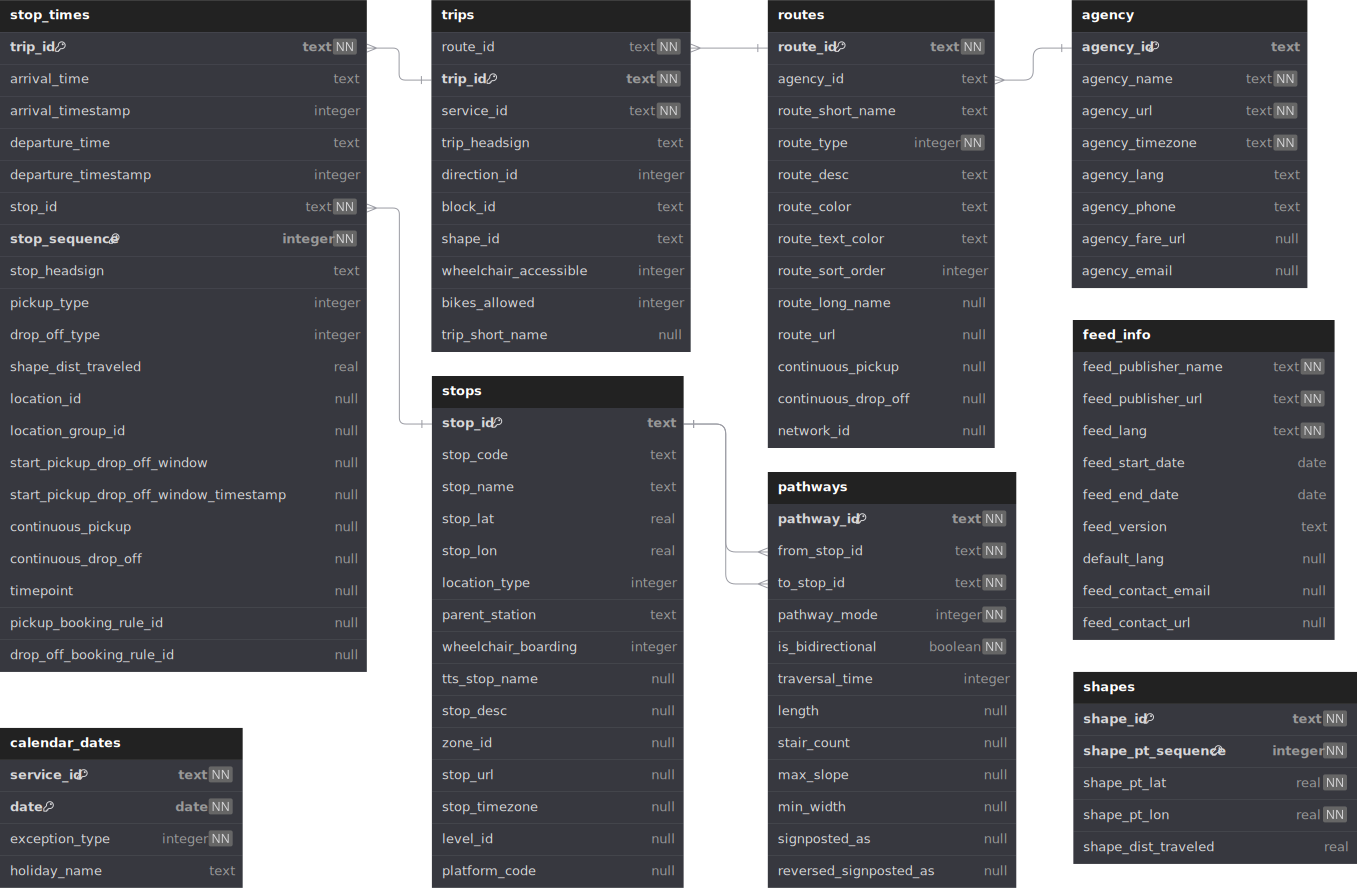
\includegraphics[width=1\textwidth]{entity_relationship}
    \caption{GTFS adatbázis sémája}
    \label{fig:gtfs-schema}
\end{figure}

\pagebreak

\textit{Megjegyzés: A teljes GTFS szabvány ennél jóval több táblát tartalmaz, de a legtöbbjük opcionális. A \ref{fig:gtfs-schema}. ábra csak azokat a táblákat tartalmazza, amelyeket a BKK OpenData Portálán elérhető adatok tartalmaznak. Ezen táblákban is vannak olyan opcionális mezők, amelyekről a BKK nem szolgáltat adatokat. Ezek a mezők a teljesség kedvéért szerepelnek a sémában, de} null \textit{típussal vannak jelölve.}

A táblák a következő információkat tartalmazzák\cite{gtfsspec}:

\begin{enumerate}
    \item \textit{agency}: A közlekedési társaságok adatait (pl. weboldal) tartalmazza. Ebben a táblában a BKK és a MÁV-HÉV adatai szerepelnek.
    \item \textit{feed\_info}: Az adatbázis verziószámát és az érvényességi időszakot tartalmazza (ez itt letöltés napjától az év végéig tart).
    \item \textit{routes}: Ez a tábla tartalmazza a járatokat (pl. 4-es villamos, 9-es busz).
    \item \textit{trips}: Ez a tábla tartalmazza a járatok útjait --- ha egy járat óránként közlekedik 9:00-tól 20:00-ig, akkor 24-szer fog szerepelni ebben a táblában: 12 oda- és ugyanennyi visszaút mindegyike egyedi azonosítóval.
    \item \textit{stop\_times}: Minden \textit{trips}-ben szereplő út egyes megállóit tartalmazza, az érkezési és indulási időpontokkal. Ez a legnagyobb tábla, jelenleg közel 6 millió rekorddal.
    \item \textit{calendar\_dates}: Arról tartalmaz információt, hogy melyik járat melyik napon lett szolgálatba állítva, illetve kiállítva. Ezt a táblát nem használjuk\footnote{A program célja nem pontos információk szolgáltatása, hanem algoritmusok demonstrálása egy ismert környezetben. Ha a cél pontos menetrendi információk megjelenítése lenne, akkor valós idejű adatokat is figyelembe kell venni, ami jelentősen növelné a program bonyolultságát, és nem tartozik a dolgozat témájába.}.
    \item \textit{shapes}: Az egyes járatok útvonalát tartalmazza pontokban; koordináta-párokat tárol, amelyeket összekötve az adott járat pontos útvonalát kapjuk a térképen. A frontend ezeket az adatokat használja az útvonalak megjelenítésére.
    \item \textit{stops}: A megállók adatait tartalmazza (pl. nevük, koordinátájuk).
    \item \textit{pathways}: Megállók közti átjárókat tartalmaz (pl. aluljárók). Ezt a táblát sem használjuk --- csak néhány átjáró van benne (jelenlegi adatok szerint 6000-nél több megállóra 500-nál kevesebb átjáró), így önmagában nem lenne elég információ az egy csoportba tartozó megállók összekötésére. Egyszerűbb és a felhasználó számára is következetesebb bármelyik 2 megálló közötti gyaloglást azonosan kezelni.
\end{enumerate}

Az adatbázis a Docker Compose fájlban mountolt \textit{data} mappába kerül, amely a \textit{frontend} és a \textit{backend} mappák mellett foglal helyet. Az alkalmazás induláskor ellenőrzi, hogy az adatbázis létezik-e (illetve sikeres-e egy lekérdezés), és ha nem, akkor betölti az adatokat a GTFS adatokból. Az adatforrás a \textit{src/configs/gtfs.config.ts} fájlban állítható be.

A gtfs könyvtár a hivatalos specifikáción felül is tartalmaz néhány segédoszlopot, amelyek a gyors lekérdezést segítik. Ezek az eredeti adatokban "óra:perc:másodperc" formátumban szereplő időpontokat egész számokká alakítják. Azonban a GTFS specifikáció szerint az éjfél után közlekedő járatok időpontjai átléphetik az "24:00:00" időpontot, amit a gtfs könyvtár nem kezel helyesen. Így betöltés után az időpontokat a programnak újra kell számolnia, hogy a betöltött adatbázisban ne null értékek legyenek.

Amint az adatbázis betöltése megtörténik, az alkalmazás GeoJson fájlokat generál a frontend számára, melyek úgyszintén a \textit{data} mappába kerülnek (\ref{fig:data-folder-structure}). Ezek a fájlok tartalmazzák a megállók és az útvonalak geometriáját\cite{rfc7946}, amelyeket a frontend a térképen megjelenít.

% dirtree?
\begin{figure}[H]
    \texttt{
        data\\
        |-- db.sqlite\\
        \'-- public\\
        \hspace{1em} |-- shapes.geo.json\\
        \hspace{1em} \'-- stops.geo.json
    }
    \caption{A \textit{data} mappa szerkezete az adatok betöltését követően}
    \label{fig:data-folder-structure}
\end{figure}

A GeoJson fájlok generálásán kívül a többi lekérdezéshez (például megállók kereséséhez) a gtfs könyvtár nem biztosít megfelelő eszközöket, így saját lekérdezéseket kell írni. Erre a \textit{Drizzle ORM} nevű könyvtárat használom, amely egy egyszerű ORM\footnote{Object-Relational Mapping, egy programozási technika, amely az objektumorientált programozást és a relációs adatbázisokat kapcsolja össze} az SQLite adatbázishoz. Azért erre esett a választásom például \textit{Prisma} helyett, mert a Drizzle csak egy vékony réteget biztosít az SQL felett\cite{drizzledocs}, így több irányításunk van a pontos lekérdezések felett, és nem kell a könyvtár által generált SQL kódot megérteni, ha egy lekérdezést optimalizálni szeretnénk. Emellett teljesítményteszteken is jobban teljesített a fent említett Prisma-nál\cite{drizzlebenchmark}. Az előnye a nyers SQL írásával szemben, hogy a Drizzle TypeScript segítségével biztosítja a típusbiztonságot, így egyszerűbb és biztonságosabb a lekérdezések írása.

\subsection{Szerkezet}

A backend osztályait és azok közötti kapcsolatokat a \ref{fig:backend-structure}. ábra mutatja be.

\begin{figure}[H]
    \centering
    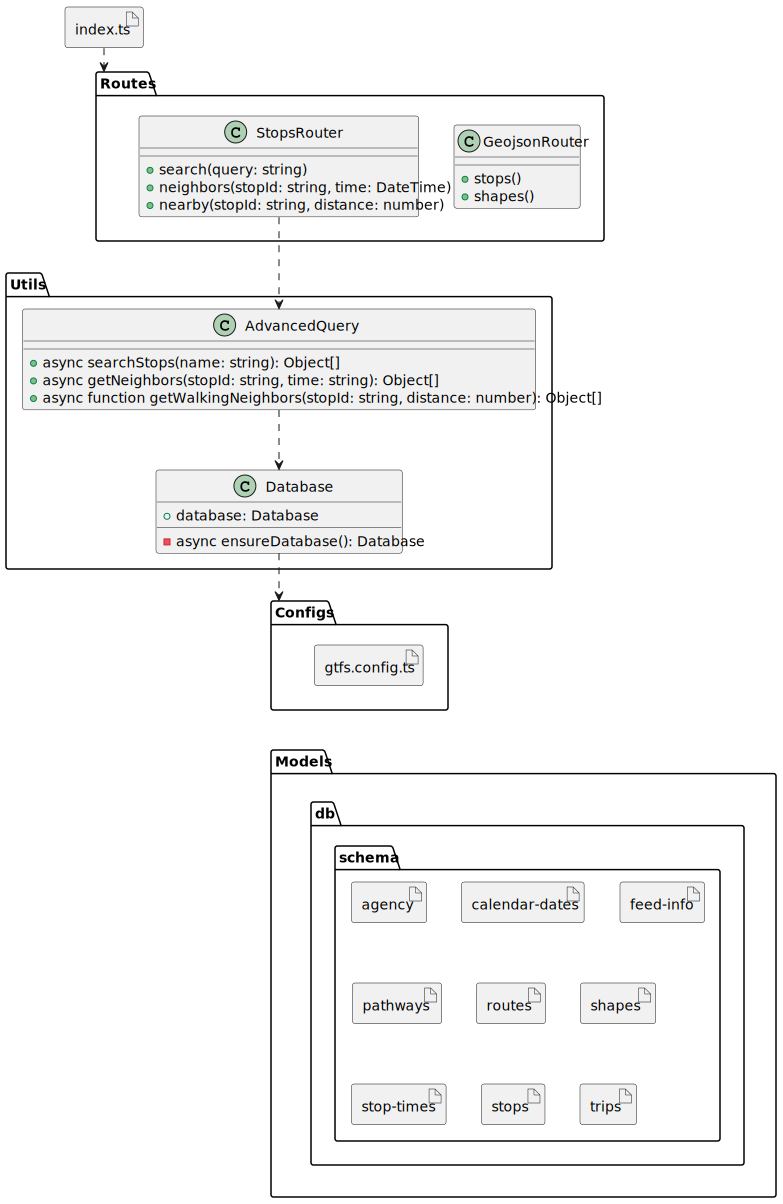
\includegraphics[width=1\textwidth]{class_backend}
    \caption{Backend szerkezete}
    \label{fig:backend-structure}
\end{figure}

\subsection{REST API}

Az alkalmazás REST API-jának végpontjai a következők:

\begin{itemize}
    \item \texttt{GET /data/stops.geo.json}: GeoJson fájl, amely a megállók koordinátáit tartalmazza.
    \item \texttt{GET /data/shapes.geo.json}: GeoJson fájl, amely az útvonalak koordinátáit tartalmazza.
    \item \texttt{GET /stops/search}: Megállók keresése név alapján.
    \item \texttt{GET /stops/:stopId/nearby}: Egy megállótól adott távolságon belüli megállók lekérdezése.
    \item \texttt{GET /stops/:stopId/neighbors}: Egy megállótól az adott időpont utáni 1 órás intervallumban induló járatokkal elérhető megállók lekérdezése.
\end{itemize}

Teljes dokumentáció sémával és példákkal a \textit{BKWay.yml} fájlban, OpenAPI 3 formátumban található.

\subsection{Tesztelés}

A backend tesztelésénél a cél az API végpontok kimerítő tesztelése volt. A tesztek futtatásához \textit{Postman}-t alkalmaztam.

A teszteléshez egy külön gtfs adatbázist használtam, mely a BKK GTFS adatbázisának egy részét tartalmazza. Erre azért volt szükség, mert az éles adatbázis bármikor változhat, és a tesztek konkrét megállók azonosítóira hagyatkoznak. Az adatbázist a backend \textit{test} mappájában található \textit{generate\_sample.sh} segítségével generáltam egy kicsomagolt GTFS-ből.

A tesztelés folyamata a következő:

\begin{enumerate}
    \item Backend konfigurálása teszt adatbázis használatára:
    \begin{compactenum}
        \item a \texttt{src/configs/gtfs.config.ts} fájlban az adatforrás átállítása a teszt zip fájlra az ott leírtak szerint
        \item a \texttt{data} mappában a \texttt{db.sqlite} fájl törlése (ha létezik)
        \item a \textit{docker-compose.debug.yml} indítása (\ref{sec:run-app})
    \end{compactenum}
    \item A Postman Collection importálása a \textit{backend/test} mappából Postman-be az \href{https://learning.postman.com/docs/getting-started/importing-and-exporting/importing-data/#import-postman-data}{itt leírtak} szerint
    \begin{compactitem}
        \item Az importáláshoz Postman fiók létrehozása szükséges.
    \end{compactitem}
    \item A tesztek futtatása a Postman-ben.
    \begin{compactitem}
        \item Az importált collection-t megnyitva, jobb felül található a "Run" gomb.
    \end{compactitem}
\end{enumerate}

\begin{figure}[H]
    \centering
    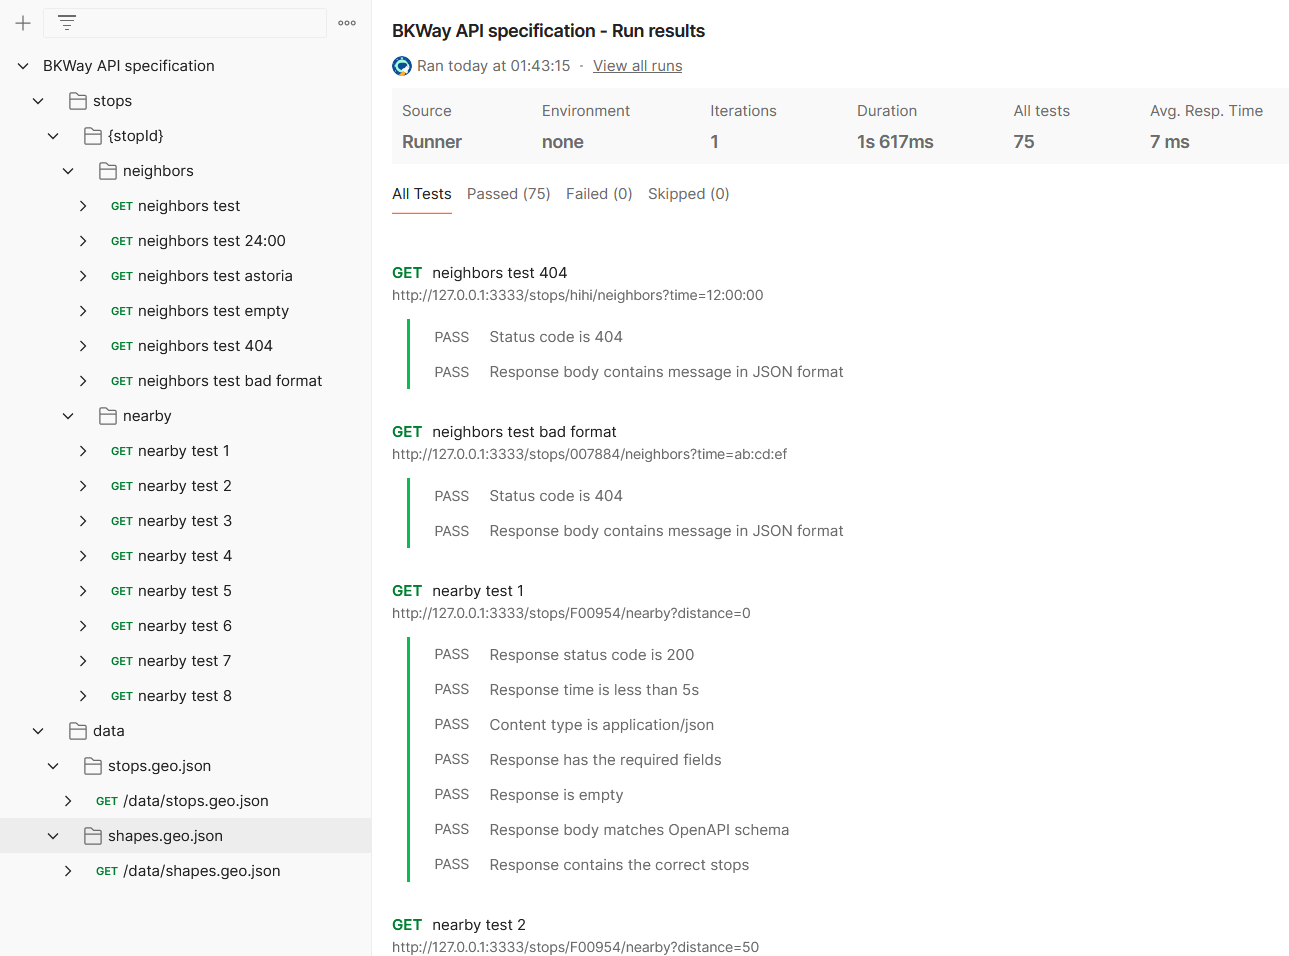
\includegraphics[width=1\textwidth]{screenshot_postman}
    \caption{Sikeres teszteredmények}
    \label{fig:screenshot-postman}
\end{figure}

A tesztek többek között a következőket ellenőrzik:
\begin{compactenum}
    \item A válasz gyorsasága
    \item A válasz státusz kódja (érvénytelen üzenetek esetén is, pl. 400 vagy 404)
    \item A válaszban szereplő pl. megállók száma
    \item A válasz megfelelése az OpenAPI sémának
\end{compactenum}

\section{Frontend}

A frontend az algoritmusok futtatásáért felelős, és a felhasználói felületet biztosítja a felhasználók számára.

\subsection{Definíciók}

\paragraph{Csúcs:} Egy gráf csúcsa egy pont a gráfban. Egy csúcsnak lehetnek szomszédos csúcsai, amelyekkel élek kötik össze. Ebben az alkalmazásban minden csúcs egy megállónak felel meg. A továbbiakban a két fogalmat szinonimaként használom.

\paragraph{Él:} Egy gráf éle egy csúcsból egy másikba mutató irányított vagy irányítatlan kapcsolat. Irányított élek esetén a két csúcs közül az egyik a kezdőpont, a másik a végpont. Egy él egy utazást reprezentál, amely egy megállóból egy másikba vezet. Az élek lehetnek súlyozatlanok és súlyozottak. Amennyiben súlyozottak, minden élhez egy súly van rendelve, ami a két csúcs közötti utazási időt jelenti. A továbbiakban "él" alatt irányított, súlyozott élt értek. Az alkalmazás szempontjából további két csoportba sorolhatók az élek: utazási élek és gyaloglási élek.

\paragraph{Utazási él:} Két megálló között közlekedő járatokat reprezentáló él. Az utazási élek súlya magában foglalja a járatra való várakozási időt is.

\paragraph{Gyaloglási él:} Két megálló közötti gyaloglást reprezentáló él. A gyaloglási élek is irányítottak.

\paragraph{Gráf:} Egy gráfot $G = (V, E)$ párként definiálunk, ahol $V$ a csúcsok halmaza, $E$ pedig az élek halmaza. Egy gráf a BKK utazási hálózatát reprezentálja.

\paragraph{Út:} Egy út egy gráfban két csúcs közötti élek sorozata. Az út bármelyik két egymást követő élére igaz, hogy ami az első él végpontja, az a másik él kezdőpontja. Az út hossza a súlyozott élek összege.

\paragraph{Útvonaltervezés:} Az útvonaltervezés (vagy \textit{útkeresés}) egy gráfban két csúcs (az induló- és a célpont) között keres utat.

\paragraph{Algoritmus:} "Algoritmus" alatt útvonaltervező algoritmusokat értek, azaz olyan utasítássorozatokat, amelyeknek a célja egy kezdő- és egy végpont közötti út megtalálása.

\paragraph{Heurisztika:} A heurisztika egy olyan $h(n)$ függvény, amely egy algoritmus számára egy becslést ad egy adott csúcsból ($n$) a célig vezető legrövidebb út hosszáról\cite{russell2020artificial}.

\subsection{Algoritmusok}
\label{ch:algo}

Az algoritmusok két fő csoportba sorolhatók: informált és informálatlan algoritmusok\cite{russell2020artificial}. Az informálatlan algoritmusok keresés közben nem veszik figyelembe a célt, csak a kezdőpontot és a gráfot járják be. Az informált algoritmusok a célt is figyelembe veszik, és ennek megfelelően működnek.

\subsubsection{BFS (Breadth-First Search) útkeresés}

A BFS algoritmus egy ún. \textit{sor} adatszerkezetet használ\cite{russell2020artificial}, ami a következő műveleteket támogatja:

\begin{compactitem}
    \item \texttt{push(elem)}: Egy elem hozzáadása a sor végéhez.
    \item \texttt{pop()}: Az első elem kivétele a sor elejéről.
\end{compactitem}

Az útkeresés a kiindulócsúcsban kezd, és a szomszédos csúcsokat egy sorba helyezi. Ezt követően minden lépésében kivesz egy csúcsot a sor elejéről, majd annak szomszédjait a sor végére helyezi. Ennek eredményeként először azokat a csúcsokat fedezi fel, amik 1 élre vannak a kiindulóponttól, majd azokat, amikhez 2 megállót kell utazni, és így tovább\cite{russell2020artificial}. Az algoritmus addig fut, amíg el nem éri a célt, vagy nincs több csúcs a sorban.

A BFS nem tesz különbséget a különböző súlyú élek között, így általában nem szokás súlyozott gráfokon alkalmazni\cite{russell2020artificial}.

Az algoritmus pszeudokódja a következő: \\

\lstset{caption={BFS algoritmus pszeudokódja}, label=src:bfs}
\begin{minipage}{\textwidth}
\begin{lstlisting}[language={Python}]
function BFS(graph, start, goal):
    queue = [start]
    visited = set()

    while queue:
        current = queue.pop()
        if current == goal:
            return current
        visited.add(current)
        for neighbor in graph[current]:
            if neighbor not in visited:
                queue.append(neighbor)
\end{lstlisting}
\end{minipage}

\subsubsection{Dijkstra algoritmus}

A Dijkstra algoritmus egy súlyozott gráfokon való legrövidebb út\cite{russell2020artificial} keresésére alkalmas algoritmus. Az algoritmus az indulási csúcsnál kezd, és a szomszédos csúcsokat egy prioritási sorban tárolja. Az algoritmus minden szomszédos csúcsot meglátogat, majd a prioritási sorból a legkisebb súlyú csúcsot veszi ki és annak szomszédjait tárolja. Mivel mindig az aktuális legkisebb súlyú csúcsot veszi ki, és egy csúcs súlya annak az időben mért távolsága az indulóállomástól, az algoritmus garantálja, hogy a célhoz vezető út a legrövidebb lesz (hiszen ha létezne rövidebb út a találtnál, azt már megtalálta volna korábban). Az algoritmus addig fut, amíg el nem éri a célt, vagy nincs több szomszédos csúcs a prioritási sorban.

Az algoritmus egy prioritási sor adatszerkezetet használ, ami a következő műveleteket támogatja:

\begin{compactitem}
    \item \texttt{insert(elem, weight)}: Egy elem hozzáadása a sorba adott súllyal.
    \item \texttt{extract\_min()}: A legkisebb elem kivétele a sorból.
\end{compactitem}

A csúcs távolságát az indulóállomásból $g(n)$ jelöli (ez az indulóállomás esetében értelemszerűen $0$). Új csúcs súlyát egy $f(n)$-nel jelölt \textit{kiértékelőfüggvény} számítja ki. mivel az algoritmus csak a távolságot veszi figyelembe, a Dijkstra algoritmusnál a kiértékelőfüggvény $f(n) = g(n)$.

Az algoritmus pszeudokódja a következő: \\

\lstset{caption={Dijkstra algoritmus pszeudokódja}, label=src:dijkstra}
\begin{minipage}{\textwidth}
\begin{lstlisting}[language={Python}]
function Dijkstra(graph, start, goal):
    pq = PriorityQueue()
    pq.insert((start, 0))
    visited = set()

    while pq:
        current, current_distance = pq.extract_min()
        if current == goal:
            return current
        visited.add(current)
        for neighbor in graph[current]:
            if neighbor not in visited:
                new_distance = current_distance + distance(current, neighbor)
                pq.insert((neighbor, new_distance))
\end{lstlisting}
\end{minipage}

\subsubsection{Mohó algoritmus}

A mohó algoritmus a Dijkstra algoritmusnak egy olyan változata, amely pusztán egy heurisztika alapján végzi az útkeresést\cite{russell2020artificial}. Ennek a kiértékelőfüggvénye $f(n) = h(n)$, ahol $h(n)$ a heurisztika értéke az adott csúcsra --- ez azt jelenti, hogy az algoritmus pusztán heurisztika alapján dönti el, hogy melyik csúcsot válassza következőnek.

A programban használt heurisztika a két pont közötti távolság a Föld\footnote{A program implementációjában a számításokhoz a \textit{distance-from} csomag szolgáltatja a távolság számításához szükséges függvényeket. Ez a könyvtár a Földet egy 6371 méter sugarú gömbként modellezi\cite{distancefrom-github}.} felszínén, egy egyenes vonalban. Ez jó választás\cite{russell2020artificial}, hiszen
\begin{compactenum}
    \item Ennél rövidebb út nem létezhet, így a heurisztika mindig alulbecsüli a távolságot, és
    \item Egyetlen képlet segítségével, gyorsan kiszámítható.
\end{compactenum}

Ez az algoritmus a legtöbb esetben sokkal gyorsabban találja meg a célt, mint a Dijkstra algoritmus, viszont nem garantálja, hogy a talált út a legrövidebb lesz --- sőt, egy olyan hálózaton, mint a tömegközlekedés, az utazási idő figyelmen kívül hagyása a tapasztalataim szerint még többet ront az eredmény minőségén, mint például egy gyalogos útvonaltervezésnél. \\

\lstset{caption={Különbség a Dijkstra és a mohó algoritmus között}, label=src:greedy}
\begin{minipage}{\textwidth}
\begin{lstlisting}[language={Python}, style=gitdiff]
function Greedy(graph, start, goal):
    pq = PriorityQueue()
    pq.insert((start, 0))
    visited = set()

    while pq:
        current, current_distance = pq.extract_min()
        if current == goal:
            return current
        visited.add(current)
        for neighbor in graph[current]:
            if neighbor not in visited:
- \-              new_distance = current_distance \+ distance(current, neighbor) -
- \-              pq.insert((neighbor, new_distance)) -
+ \+              pq.insert((neighbor, heuristic(neighbor))) +
\end{lstlisting}
\end{minipage}

\subsubsection{A* algoritmus}

Az A* algoritmus\footnote{A szakirodalomban az A* algoritmus nem mindig tartalmazza a heurisztika súlyozását, ilyenkor ezt a változatot \textit{súlyozott A*}-nak nevezik\cite{russell2020artificial}. Én az egyszerűség kedvéért erre a variánsra egyszerűen A*-ként hivatkozom, a "súlyozatlan" változatot pedig a továbbiakban nem említem meg.} a Dijkstra és a mohó algoritmusok kombinációja, amely a Dijkstra algoritmus pontosságát ötvözi a mohó algoritmus gyorsaságával. Ezt úgy éri el, hogy a prioritási sor elemeit a súlyok és a súlyozott heurisztika összege szerint rendezi.

"Súlyozott heurisztika" alatt egyszerűen a heurisztika és egy $W$ súly szorzatát értem. Az A* kiértékelőfüggvénye tehát a következő\cite{russell2020artificial}:

$$f(n) = g(n) + W \times h(n)$$

A súly értékének változtatásával az algoritmus többet vagy kevesebbet fog támaszkodni a heurisztikára, tehát a súly csökkentéséhez közelebb kerülhetünk a Dijkstra algoritmushoz pontos eredményeihez, míg a súly növelésével a mohó algoritmus gyorsaságához.

Az algoritmus pszeudokódja a következő: \\

\lstset{caption={Különbség a Dijkstra és az A* algoritmus között}, label=src:astar}
\begin{minipage}{\textwidth}
\begin{lstlisting}[language={Python}, style=gitdiff]
function Greedy(graph, start, goal):
    pq = PriorityQueue()
    pq.insert((start, 0))
    visited = set()

    while pq:
        current, current_distance = pq.extract_min()
        if current == goal:
            return current
        visited.add(current)
        for neighbor in graph[current]:
            if neighbor not in visited:
                new_distance = current_distance \+ distance(current, neighbor)
- \-              pq.insert((neighbor, new_distance)) -
+ \+              pq.insert((neighbor, new_distance \+ heuristic(neighbor))) +
\end{lstlisting}
\end{minipage}

\section{Implementáció}

\subsection{Algoritmusok}

Megfigyelhető, hogy az algoritmusok szerkezetükben nagyon hasonlóak egymáshoz. A prioritási sor-alapú algoritmusok esetében egyértelmű, hiszen csak egy-két sor változtatásra vannak egymástól, ám a BFS sem különbözik sokban ezektől. Néhány triviális változó- illetve metódus-átnevezés után a \ref{src:dijkstra-diff}. kódrészletben látható, hogy a BFS és a mohó algoritmus mennyire hasonlít. \\

\lstset{
    caption={Különbségek a Dijkstra és a mohó algoritmus pszeudokódja között},
    label=src:dijkstra-diff,
    escapechar=§}
\begin{minipage}{\textwidth}
\begin{lstlisting}[language={Python}, style=gitdiff]

- \-  function BFS(graph, start, goal): -
+ \+  function Dijkstra(graph, start, goal): +
- \-      queue = Queue() -
+ \+      queue = PriorityQueue() +

- \-      queue.insert(start) -
+ \+      queue.insert((start, 0)) +
        visited = set()

        while queue:
- \-          current = queue.pop() -
+ \+          current, current_distance = queue.pop() +
            if current == goal:
                return current
            visited.add(current)
            for neighbor in graph[current]:
                if neighbor not in visited:
- \-                  queue.insert(neighbor) -
+ \+                  queue.insert((neighbor, heuristic(neighbor))) +
\end{lstlisting}
\end{minipage}

Mint látható, a program folyása teljes azonos köztük, az egyetlen különbség, hogy a prioritási sor alapú algoritmusok súlyt társítanak a sor elemeihez. Ez azt jelenti, hogy akár a BFS algoritmust is át lehetne írni úgy, hogy prioritási sort használjon, ha a minden csúcs súlyát eggyel nagyobbra állítanánk az előzőénél, hiszen így garantáltan a prioritási sor végére kerülne. Ezt egyszerűen el lehetne érni, hiszen az összes ismert csúcs száma soha nem csökken, és a p. sorba\footnote{Prioritási sor} való beillesztéskor mindig a p. sor hosszának és a látogatott csúcsok számának az összege.

Bár ez működne, hatékonysági megfontolásból nem emellett a megoldás mellett döntöttem. Helyette az algoritmusokat megvalósító absztrakt osztályhoz egy absztrakt \textit{data} adattagot vettem fel. Ennek típusa, az \textit{IDataStructure} interfész néhány alapvető függvényt tartalmaz; többek közt az új elem hozzáadását és az elem kivételét. A heurisztika, forrástól való távolság, és hasonló információk egy csúcsról az útkereső osztály helyett a csúcs (\textit{Vertex}) osztályban kerülnek kiszámításra, így az útkeresés (\textit{Pathfinding}) szabadon használhatja ezeket.

\begin{figure}[H]
    \centering
    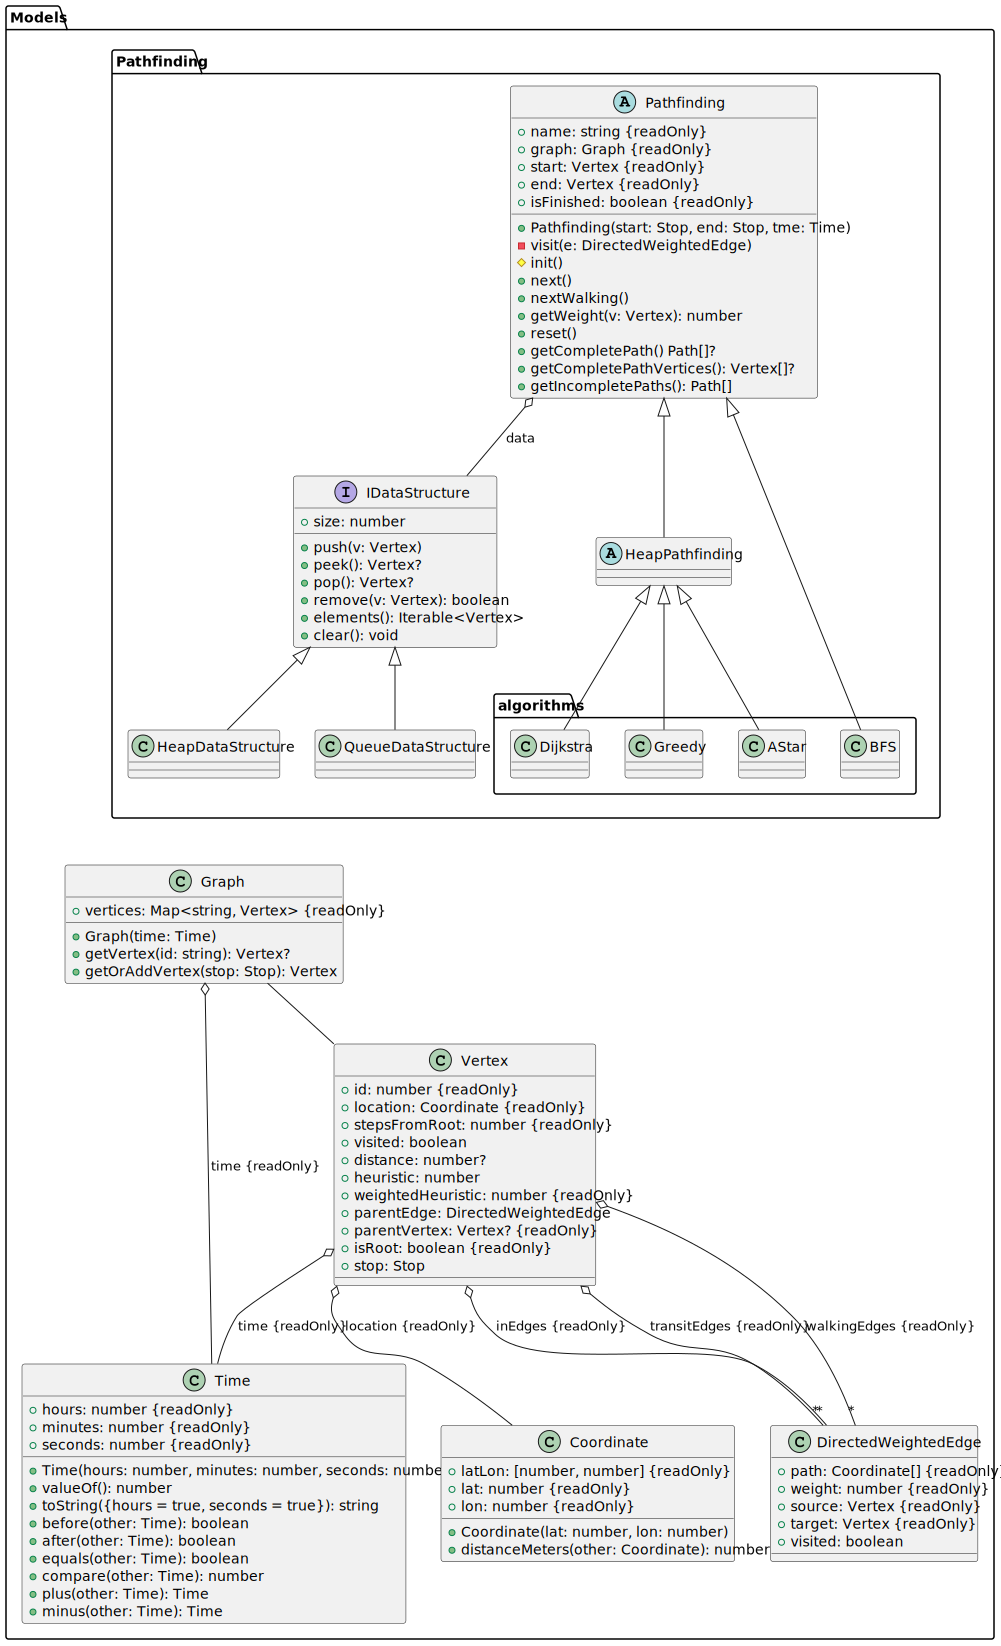
\includegraphics[width=1\textwidth]{class_frontend_models}
    \caption{Frontend modellek}
    \label{fig:frontend-models}
\end{figure}

\subsection{Felhasználói felület}

A felhasználói felület React komponenseket használ, amelyek a \textit{Material UI} React komponens könyvtár komponenseivel épülnek fel. Ez a könyvtár előre elkészített, egységes dizájnelemeket tartalmaz, amelyek a Google Material Design irányelvei alapján készültek\cite{mui}. A Material UI-hoz kapcsolódó \textit{MUI X} könyvtár az indulási idő beállításához használt \textit{TimePicker} komponenst biztosítja. A felhasználói felület főbb komponensei a \ref{fig:screenshot-components-settings}. és \ref{fig:screenshot-components-route}. ábrákon láthatóak.

\begin{figure}[H]
    \centering
    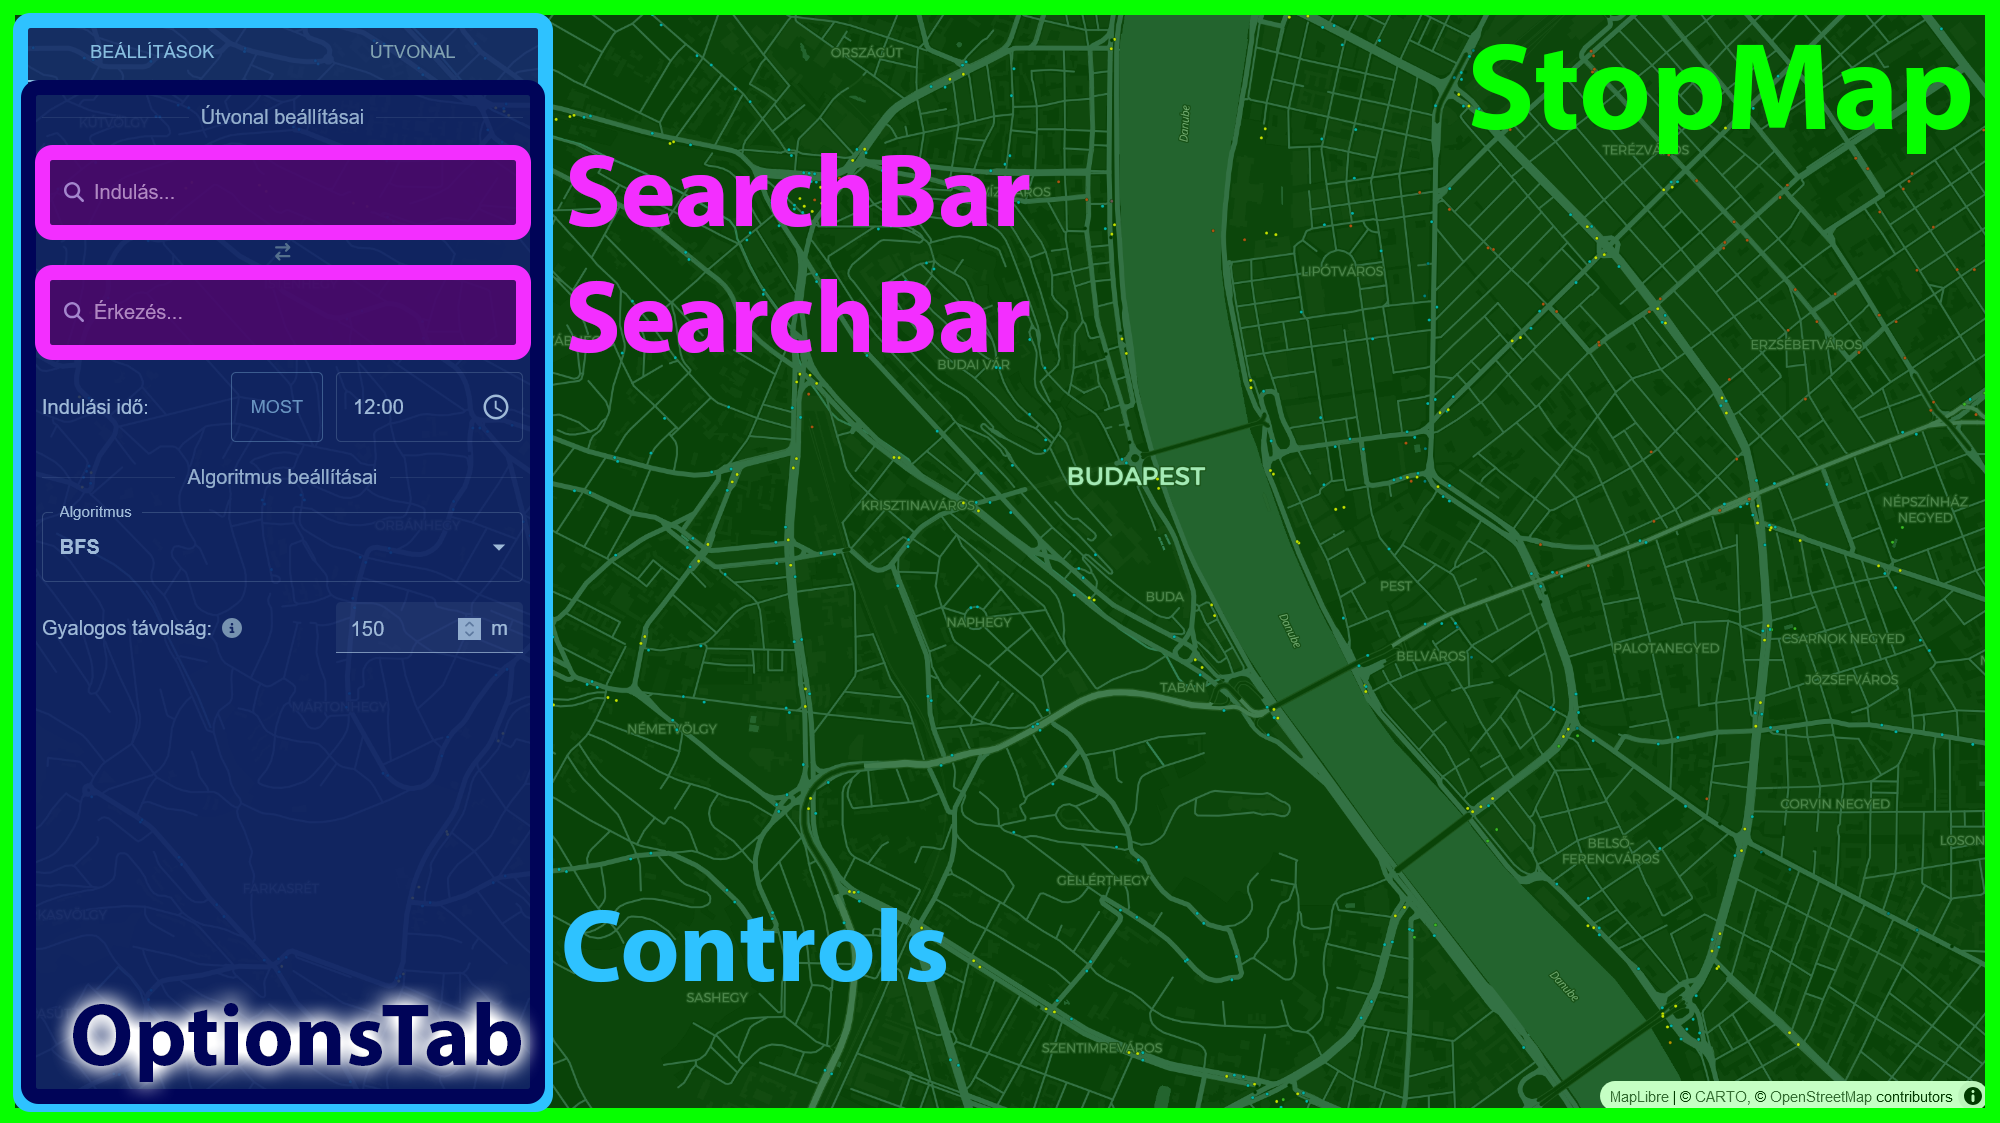
\includegraphics[width=1\textwidth]{screenshot_components_settings}
    \caption{Beállítások komponense}
    \label{fig:screenshot-components-settings}
\end{figure}

\begin{figure}[H]
    \centering
    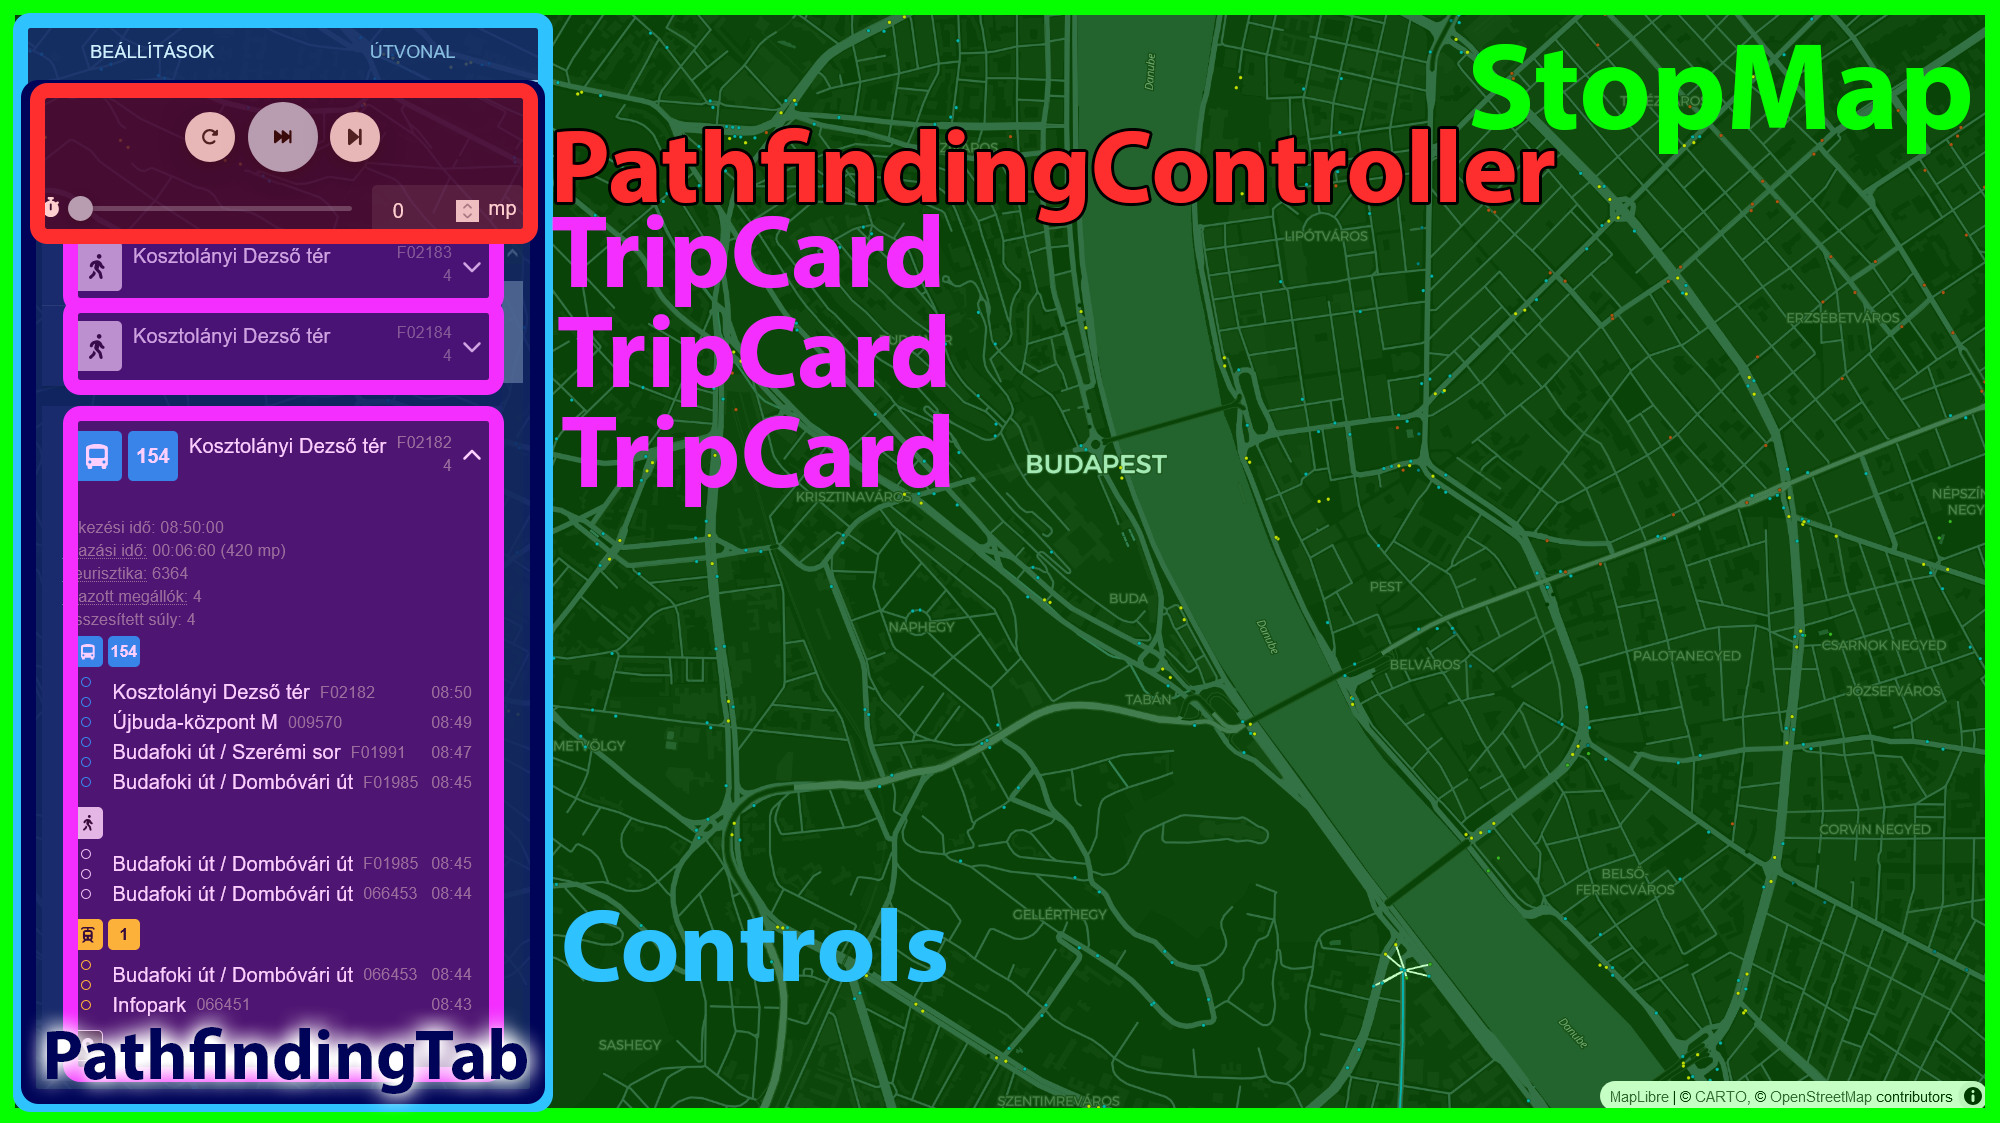
\includegraphics[width=1\textwidth]{screenshot_components_route}
    \caption{Keresés komponense}
    \label{fig:screenshot-components-route}
\end{figure}

\textit{Megjegyzés: A} StopMap \textit{komponenes nem tartalmazza magában a} Controls \textit{komponenst,} de a többi komponens egymásba ágyazása úgy történik, ahogy vizuálisan látható --- A \textit{Controls} foglalja magában a bal oldali irányítópanel összes elemét, ezen belül az \textit{OptionsTab} és a \textit{PathfindingTab} komponenseket, melyek a két fül elemeit tartalmazzák.

\subsection{API hívások}

Az API hívásokért az \textit{api.service.ts} felel, amely \textit{fetch} hívásokkal kommunikál a backenddel. A visszatérési típusok a backendben definiált adatbázis sémájából lettek generálva, így megegyeznek a backend által küldött adatok típusával.

\subsection{Tesztelés}

Az útvonaltervezés tesztelése manuálisan történik, néhány példaútvonalon keresztül. Minden útvonaltervezést \textit{12:00}-kor kezdünk, ha nem szerepel más időpont. A sétálási távolságot is hagyjuk az alapértelmezett 150 méteren, ha nem szerepel más érték.

\subsubsection{Útkeresés önmagába}

Adjuk meg induló- és érkező állomásnak is ugyanazt az állomást. Erre jó alany a \textit{Csobánc utca}, mert ilyen nevű állomásból csak egy van a térképen. Ekkor egyik algoritmusnak sem szabad elindulnia, és azonnal jelezniük kell, hogy megtalálta a célt.

\subsubsection{BFS útkeresés}

A BFS nem veszi figyelembe az élek súlyát, csak a megállók számát. Tervezzünk utat a \textit{Népliget} (\textit{F01282}\footnote{Az indulási- és érkezési megállók azonosítója a kiválasztást követően a böngésző konzolában is megjelenik}) és a \textit{Kőris utca (Korányi Sándor utca)} megállók között 175m gyaloglási távolsággal. Az algoritmusnak hamarabb kell felfedeznie a Kálvin tér-ből induló járatokat, mint megtalálnia a célállomást, hiszen az M3 vonalán ez ugyanúgy 4 megállóra van, mint a 83-as vonalán a Kőris utca (Korányi Sándor utca) megálló, és az M3 indulóállomásából terveztünk utat. Az algoritmusnak a 83-as trolival kell eljutnia a célállomásra.

\subsubsection{Dijkstra útkeresés}

Használjuk a BFS beállításait. A Dijkstra algoritmusnak hamarabb kell hozzáadnia a Deák Ferenc tér (\textit{F00954}) M3 metrómegállót a prioritási sorba, mint megtalálnia az utat, de nem szabad a Kálvin tér többi megállóját meglátogatnia (ami nem az M3 megállója), mert azokhoz több idő sétálni, mint a célállomásra.

\subsubsection{Mohó útkeresés}

A mohó útvonaltervezés gyakorlatilag bármilyen útvonalon ellenőrizhető, mert látványosan figyelmen kívül hagyja az utazási időt (ellenben a távolsággal). Tervezzünk utat Ráckeve és Szentendre között. Az útkeresés belátható időn belül végezni fog, és nem fedezi fel Budapest nagy részét, mielőtt célba ér.

\subsubsection{A* útkeresés}

Az A* algoritmus tesztelésekor fontos, hogy a súlyozott heurisztika helyesen működjön. Tervezzünk utat a \textit{Margit híd, budai hídfő H} (\textit{F00189}) és a \textit{Petőfi híd, budai hídfő} (\textit{F02224}) megállók között, ahol megáll a 4-es és a 6-os villamos. Az algoritmus $0.3\times$ heurisztika súly esetén a 4-es vagy 6-os villamossal fogja megtalálni a célt. $0.7\times$ súly esetén az út Budapest \textit{Kiskörút}ján fog áthaladni, részben a 9-es busz vonalán. $2.5\times$ súly esetén a talált út a 15-ös busz vonalán lévő a \textit{Kossuth Lajos tér M} és a \textit{Petőfi tér} megállókat is tartalmazni fogja.

\section{Telepítés}

A programot az itthoni szerveremen futtatom, jelenleg a \mbox{\url{https://bee-612.space/bkway/}} címen elérhető. Más szerveren való futtatáshoz a \ref{sec:run-app} alatt található használati utasítást kell követni, illetve a következő helyeken a megfelelő változókat beállítani:

\begin{itemize}
    \item A \textit{docker-compose.yml} fájlban a bkway-back szolgáltatásnál a \texttt{BKWAY\_FRONTEND} környezeti változót a frontend domainjére állítani,
    \item a frontend \textit{.env} fájljában a \texttt{BKWAY\_BACKEND} változót a backend címére állítani,
    \item végül opcionálisan a frontend \textit{vite.config.ts} fájljában a konfiguráció \texttt{base} értékét átállítani. Jelenlegi értéke \textit{/bkway/}, ami azt jelenti, hogy a \mbox{\texttt{https://your.domain.com/bkway/}} elérési úton lesz kiszolgálva.
\end{itemize}

\section{További fejlesztési lehetőségek}

\subsubsection{Adatbázis lekérdezések gyorsítása}

Jelenleg a megállókra való keresésnél az adatbázis lekérdezés költséges táblaösszekapcsolásokat végez el. Bár ezeknek az eredménye gyorsítótárazva van a szerveren, még sokszor lehetnek lassúak a lekérdezések. Mivel az adatbázis nem változik a létrehozása után, nem lenne nehéz egy kapcsolótábla létrehozása, ami a \textit{stops} és a \textit{routes} táblát köti össze. Ezzel azt gondolom, hogy a lekérdezések 10-100-szoros gyorsulást érhetnének el.

\subsubsection{Animáció gyorsítása}

Jelenleg a frontend az útvonaltervezés minden egyes lépése után újra kiszámítja a forrásból az összes sorban szereplő elembe vezető utat. Ez hosszú sor és folyamatos animáció esetén lassú tud lenni. Ha az algoritmus számon tartaná az egy lépésen belül történt változtásokat, és csak azokat frissítené, akkor a program jelentősen gyorsabb lenne.

\subsubsection{További részletek megjelenítése}

Jelenleg a felhasználói felület "ÚTVONAL" fülén csak a felfedezésre váró megállók és az azokhoz tartozó információk jelennek meg. Hasznos információ lenne itt többek között az algoritmus által megtett lépések száma és a már felfedezett megállók (akár kereshető) listája is.

\subsubsection{Új algoritmusok hozzáadása}

Az A* algoritmus egy gyakori példa hatékony útvonaltervezésre, de elérhetőek újabb, modernebb és hatékonyabb algoritmusok is. Ilyen például a RAPTOR\cite{raptor}, amely különösen tömegközlekedési hálózatokra van kifejlesztve, vagy egyszerűen az A* algoritmus súlyozott változata.

\subsubsection{Új beállítások hozzáadása}

További hasznos beállítások lehetnek az átszállások száma, a tömegközlekedési eszközök szűrése, vagy az akadálymentes útvonaltervezés.

\subsubsection{Valós idejű adatok megjelenítése}

A BKK Futár API GTFS-Realtime formátumban szolgáltat valós idejű adatokat a járatokról\cite{bkkopendata}, amelyeket fel lehetne használni az útvonaltervezés során.
